\chapter{Flows and cuts}

In this chapter, we focus on the following
two problems:

\begin{itemize}
\item \key{Finding a maximum flow}:
What is the maximum amount of flow we can
send from a node to another node?
\item \key{Finding a minimum cut}:
What is a minimum-weight set of edges
that separates two nodes of the graph?
\end{itemize}

The input for both these problems is a directed,
weighted graph that contains two special nodes:
the \emph{source} is a node with no incoming edges,
and the \emph{sink} is a node with no outgoing edges.

As an example, we will use the following graph
where node 1 is the source and node 6
is the sink:

\begin{center}
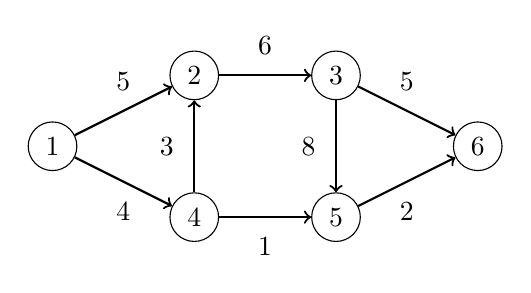
\begin{tikzpicture}[scale=0.9]
\node[draw, circle] (1) at (1,2) {$1$};
\node[draw, circle] (2) at (3,3) {$2$};
\node[draw, circle] (3) at (5,3) {$3$};
\node[draw, circle] (4) at (7,2) {$6$};
\node[draw, circle] (5) at (3,1) {$4$};
\node[draw, circle] (6) at (5,1) {$5$};
\path[draw,thick,->] (1) -- node[font=\small,label=5] {} (2);
\path[draw,thick,->] (2) -- node[font=\small,label=6] {} (3);
\path[draw,thick,->] (3) -- node[font=\small,label=5] {} (4);
\path[draw,thick,->] (1) -- node[font=\small,label=below:4] {} (5);
\path[draw,thick,->] (5) -- node[font=\small,label=below:1] {} (6);
\path[draw,thick,->] (6) -- node[font=\small,label=below:2] {} (4);
\path[draw,thick,<-] (2) -- node[font=\small,label=left:3] {} (5);
\path[draw,thick,->] (3) -- node[font=\small,label=left:8] {} (6);
\end{tikzpicture}
\end{center}

\subsubsection{Maximum flow}

\index{flow}
\index{maximum flow}

In the \key{maximum flow} problem,
our task is to send as much flow as possible
from the source to the sink.
The weight of each edge is a capacity that
restricts the flow
that can go through the edge.
In each intermediate node,
the incoming and outgoing
flow has to be equal.

For example, the maximum size of a flow
in the example graph is 7.
The following picture shows how we can
route the flow:

\begin{center}
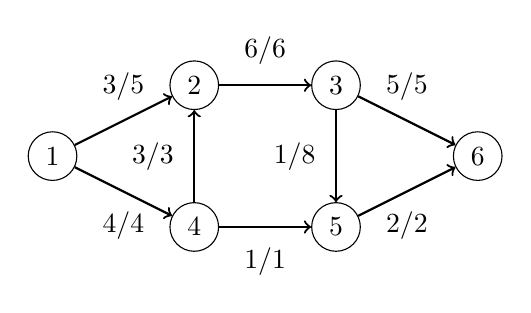
\begin{tikzpicture}[scale=0.9]
\node[draw, circle] (1) at (1,2) {$1$};
\node[draw, circle] (2) at (3,3) {$2$};
\node[draw, circle] (3) at (5,3) {$3$};
\node[draw, circle] (4) at (7,2) {$6$};
\node[draw, circle] (5) at (3,1) {$4$};
\node[draw, circle] (6) at (5,1) {$5$};
\path[draw,thick,->] (1) -- node[font=\small,label=3/5] {} (2);
\path[draw,thick,->] (2) -- node[font=\small,label=6/6] {} (3);
\path[draw,thick,->] (3) -- node[font=\small,label=5/5] {} (4);
\path[draw,thick,->] (1) -- node[font=\small,label=below:4/4] {} (5);
\path[draw,thick,->] (5) -- node[font=\small,label=below:1/1] {} (6);
\path[draw,thick,->] (6) -- node[font=\small,label=below:2/2] {} (4);
\path[draw,thick,<-] (2) -- node[font=\small,label=left:3/3] {} (5);
\path[draw,thick,->] (3) -- node[font=\small,label=left:1/8] {} (6);
\end{tikzpicture}
\end{center}

The notation $v/k$ means
that a flow of $v$ units is routed through
an edge whose capacity is $k$ units.
The size of the flow is $7$,
because the source sends $3+4$ units of flow
and the sink receives $5+2$ units of flow.
It is easy see that this flow is maximum,
because the total capacity of the edges
leading to the sink is $7$.

\subsubsection{Minimum cut}

\index{cut}
\index{minimum cut}

In the \key{minimum cut} problem,
our task is to remove a set
of edges from the graph
such that there will be no path from the source
to the sink after the removal
and the total weight of the removed edges
is minimum.

The minimum size of a cut in the example graph is 7.
It suffices to remove the edges $2 \rightarrow 3$
and $4 \rightarrow 5$:

\begin{center}
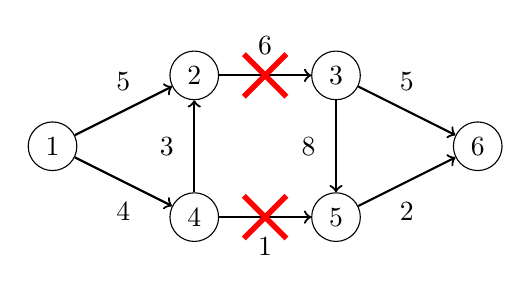
\begin{tikzpicture}[scale=0.9]
\node[draw, circle] (1) at (1,2) {$1$};
\node[draw, circle] (2) at (3,3) {$2$};
\node[draw, circle] (3) at (5,3) {$3$};
\node[draw, circle] (4) at (7,2) {$6$};
\node[draw, circle] (5) at (3,1) {$4$};
\node[draw, circle] (6) at (5,1) {$5$};
\path[draw,thick,->] (1) -- node[font=\small,label=5] {} (2);
\path[draw,thick,->] (2) -- node[font=\small,label=6] {} (3);
\path[draw,thick,->] (3) -- node[font=\small,label=5] {} (4);
\path[draw,thick,->] (1) -- node[font=\small,label=below:4] {} (5);
\path[draw,thick,->] (5) -- node[font=\small,label=below:1] {} (6);
\path[draw,thick,->] (6) -- node[font=\small,label=below:2] {} (4);
\path[draw,thick,<-] (2) -- node[font=\small,label=left:3] {} (5);
\path[draw,thick,->] (3) -- node[font=\small,label=left:8] {} (6);

\path[draw=red,thick,-,line width=2pt] (4-.3,3-.3) -- (4+.3,3+.3);
\path[draw=red,thick,-,line width=2pt] (4-.3,3+.3) -- (4+.3,3-.3);
\path[draw=red,thick,-,line width=2pt] (4-.3,1-.3) -- (4+.3,1+.3);
\path[draw=red,thick,-,line width=2pt] (4-.3,1+.3) -- (4+.3,1-.3);
\end{tikzpicture}
\end{center}

After removing the edges,
there will be no path from the source to the sink.
The size of the cut is $7$,
because the weights of the removed edges
are $6$ and $1$.
The cut is minimum, because there is no valid
way to remove edges from the graph such that
their total weight would be less than $7$.
\\\\
It is not a coincidence that
the maximum size of a flow
and the minimum size of a cut
are the same in the above example.
It turns out that a maximum flow
and a minimum cut are
\emph{always} equally large,
so the concepts are two sides of the same coin.

Next we will discuss the Ford–Fulkerson
algorithm that can be used to find
the maximum flow and minimum cut of a graph.
The algorithm also helps us to understand
\emph{why} they are equally large.

\section{Ford–Fulkerson algorithm}

\index{Ford–Fulkerson algorithm}

The \key{Ford–Fulkerson algorithm} \cite{for56} finds
the maximum flow in a graph.
The algorithm begins with an empty flow,
and at each step finds a path from the source
to the sink that generates more flow.
Finally, when the algorithm cannot increase the flow
anymore, the maximum flow has been found.

The algorithm uses a special representation
of the graph where each original edge has a reverse
edge in another direction.
The weight of each edge indicates how much more flow
we could route through it.
At the beginning of the algorithm, the weight of each original edge
equals the capacity of the edge
and the weight of each reverse edge is zero.

\begin{samepage}
The new representation for the example graph is as follows:

\begin{center}
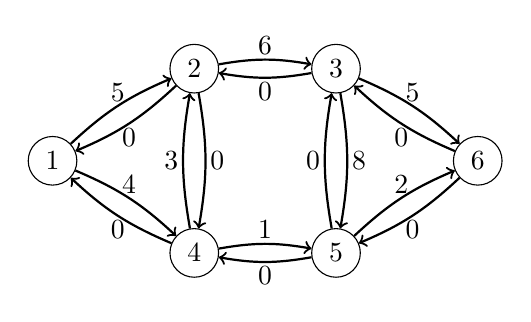
\begin{tikzpicture}[scale=0.9,label distance=-2mm]
\node[draw, circle] (1) at (1,1.3) {$1$};
\node[draw, circle] (2) at (3,2.6) {$2$};
\node[draw, circle] (3) at (5,2.6) {$3$};
\node[draw, circle] (4) at (7,1.3) {$6$};
\node[draw, circle] (5) at (3,0) {$4$};
\node[draw, circle] (6) at (5,0) {$5$};

\path[draw,thick,->] (1) edge [bend left=10] node[font=\small,label=5] {} (2);
\path[draw,thick,->] (2) edge [bend left=10] node[font=\small,label=below:0] {} (1);
\path[draw,thick,->] (2) edge [bend left=10] node[font=\small,label=6] {} (3);
\path[draw,thick,->] (3) edge [bend left=10] node[font=\small,label=below:0] {} (2);
\path[draw,thick,->] (3) edge [bend left=10] node[font=\small,label=5] {} (4);
\path[draw,thick,->] (4) edge [bend left=10] node[font=\small,label=below:0] {} (3);
\path[draw,thick,->] (1) edge [bend left=10] node[font=\small,label=4] {} (5);
\path[draw,thick,->] (5) edge [bend left=10] node[font=\small,label=below:0] {} (1);
\path[draw,thick,->] (5) edge [bend left=10] node[font=\small,label=1] {} (6);
\path[draw,thick,->] (6) edge [bend left=10] node[font=\small,label=below:0] {} (5);
\path[draw,thick,->] (6) edge [bend left=10] node[font=\small,label=2] {} (4);
\path[draw,thick,->] (4) edge [bend left=10] node[font=\small,label=below:0] {} (6);
\path[draw,thick,->] (5) edge [bend left=10] node[font=\small,label=left:3] {} (2);
\path[draw,thick,->] (2) edge [bend left=10] node[font=\small,label=right:0] {} (5);
\path[draw,thick,->] (3) edge [bend left=10] node[font=\small,label=right:8] {} (6);
\path[draw,thick,->] (6) edge [bend left=10] node[font=\small,label=left:0] {} (3);
\end{tikzpicture}
\end{center}
\end{samepage}

\subsubsection{Algorithm description}

The Ford–Fulkerson algorithm consists of several
rounds.
On each round, the algorithm finds
a path from the source to the sink
such that each edge on the path has a positive weight.
If there is more than one possible path available,
we can choose any of them.

For example, suppose we choose the following path:

\begin{center}
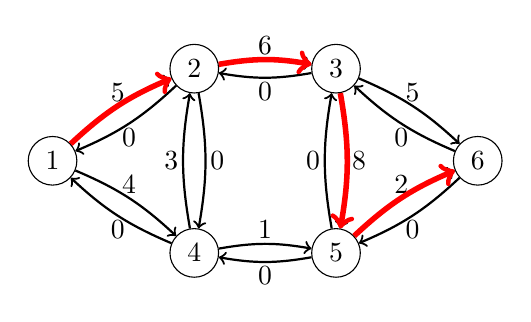
\begin{tikzpicture}[scale=0.9,label distance=-2mm]
\node[draw, circle] (1) at (1,1.3) {$1$};
\node[draw, circle] (2) at (3,2.6) {$2$};
\node[draw, circle] (3) at (5,2.6) {$3$};
\node[draw, circle] (4) at (7,1.3) {$6$};
\node[draw, circle] (5) at (3,0) {$4$};
\node[draw, circle] (6) at (5,0) {$5$};

\path[draw,thick,->] (1) edge [bend left=10] node[font=\small,label=5] {} (2);
\path[draw,thick,->] (2) edge [bend left=10] node[font=\small,label=below:0] {} (1);
\path[draw,thick,->] (2) edge [bend left=10] node[font=\small,label=6] {} (3);
\path[draw,thick,->] (3) edge [bend left=10] node[font=\small,label=below:0] {} (2);
\path[draw,thick,->] (3) edge [bend left=10] node[font=\small,label=5] {} (4);
\path[draw,thick,->] (4) edge [bend left=10] node[font=\small,label=below:0] {} (3);
\path[draw,thick,->] (1) edge [bend left=10] node[font=\small,label=4] {} (5);
\path[draw,thick,->] (5) edge [bend left=10] node[font=\small,label=below:0] {} (1);
\path[draw,thick,->] (5) edge [bend left=10] node[font=\small,label=1] {} (6);
\path[draw,thick,->] (6) edge [bend left=10] node[font=\small,label=below:0] {} (5);
\path[draw,thick,->] (6) edge [bend left=10] node[font=\small,label=2] {} (4);
\path[draw,thick,->] (4) edge [bend left=10] node[font=\small,label=below:0] {} (6);
\path[draw,thick,->] (5) edge [bend left=10] node[font=\small,label=left:3] {} (2);
\path[draw,thick,->] (2) edge [bend left=10] node[font=\small,label=right:0] {} (5);
\path[draw,thick,->] (3) edge [bend left=10] node[font=\small,label=right:8] {} (6);
\path[draw,thick,->] (6) edge [bend left=10] node[font=\small,label=left:0] {} (3);

\path[draw=red,thick,->,line width=2pt] (1) edge [bend left=10] (2);
\path[draw=red,thick,->,line width=2pt] (2) edge [bend left=10] (3);
\path[draw=red,thick,->,line width=2pt] (3) edge [bend left=10] (6);
\path[draw=red,thick,->,line width=2pt] (6) edge [bend left=10] (4);
\end{tikzpicture}
\end{center}

After choosing the path, the flow increases by $x$ units,
where $x$ is the smallest edge weight on the path.
In addition, the weight of each edge on the path
decreases by $x$ and the weight of each reverse edge
increases by $x$.

In the above path, the weights of the
edges are 5, 6, 8 and 2.
The smallest weight is 2,
so the flow increases by 2
and the new graph is as follows:

\begin{center}
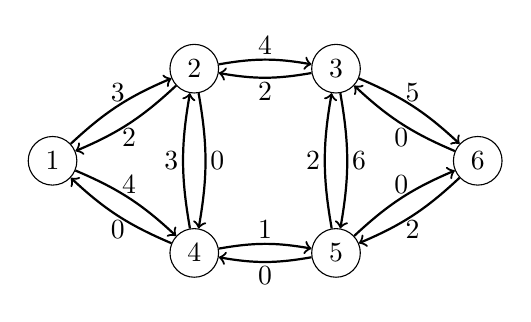
\begin{tikzpicture}[scale=0.9,label distance=-2mm]
\node[draw, circle] (1) at (1,1.3) {$1$};
\node[draw, circle] (2) at (3,2.6) {$2$};
\node[draw, circle] (3) at (5,2.6) {$3$};
\node[draw, circle] (4) at (7,1.3) {$6$};
\node[draw, circle] (5) at (3,0) {$4$};
\node[draw, circle] (6) at (5,0) {$5$};

\path[draw,thick,->] (1) edge [bend left=10] node[font=\small,label=3] {} (2);
\path[draw,thick,->] (2) edge [bend left=10] node[font=\small,label=below:2] {} (1);
\path[draw,thick,->] (2) edge [bend left=10] node[font=\small,label=4] {} (3);
\path[draw,thick,->] (3) edge [bend left=10] node[font=\small,label=below:2] {} (2);
\path[draw,thick,->] (3) edge [bend left=10] node[font=\small,label=5] {} (4);
\path[draw,thick,->] (4) edge [bend left=10] node[font=\small,label=below:0] {} (3);
\path[draw,thick,->] (1) edge [bend left=10] node[font=\small,label=4] {} (5);
\path[draw,thick,->] (5) edge [bend left=10] node[font=\small,label=below:0] {} (1);
\path[draw,thick,->] (5) edge [bend left=10] node[font=\small,label=1] {} (6);
\path[draw,thick,->] (6) edge [bend left=10] node[font=\small,label=below:0] {} (5);
\path[draw,thick,->] (6) edge [bend left=10] node[font=\small,label=0] {} (4);
\path[draw,thick,->] (4) edge [bend left=10] node[font=\small,label=below:2] {} (6);
\path[draw,thick,->] (5) edge [bend left=10] node[font=\small,label=left:3] {} (2);
\path[draw,thick,->] (2) edge [bend left=10] node[font=\small,label=right:0] {} (5);
\path[draw,thick,->] (3) edge [bend left=10] node[font=\small,label=right:6] {} (6);
\path[draw,thick,->] (6) edge [bend left=10] node[font=\small,label=left:2] {} (3);
\end{tikzpicture}
\end{center}

The idea is that increasing the flow decreases the amount of
flow that can go through the edges in the future.
On the other hand, it is possible to cancel
flow later using the reverse edges of the graph
if it turns out that
it would be beneficial to route the flow in another way.

The algorithm increases the flow as long as
there is a path from the source
to the sink through positive-weight edges.
In the present example, our next path can be as follows:

\begin{center}
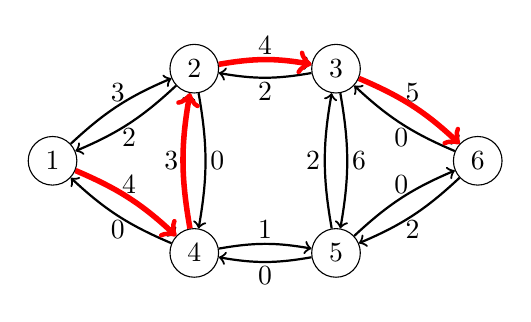
\begin{tikzpicture}[scale=0.9,label distance=-2mm]
\node[draw, circle] (1) at (1,1.3) {$1$};
\node[draw, circle] (2) at (3,2.6) {$2$};
\node[draw, circle] (3) at (5,2.6) {$3$};
\node[draw, circle] (4) at (7,1.3) {$6$};
\node[draw, circle] (5) at (3,0) {$4$};
\node[draw, circle] (6) at (5,0) {$5$};

\path[draw,thick,->] (1) edge [bend left=10] node[font=\small,label=3] {} (2);
\path[draw,thick,->] (2) edge [bend left=10] node[font=\small,label=below:2] {} (1);
\path[draw,thick,->] (2) edge [bend left=10] node[font=\small,label=4] {} (3);
\path[draw,thick,->] (3) edge [bend left=10] node[font=\small,label=below:2] {} (2);
\path[draw,thick,->] (3) edge [bend left=10] node[font=\small,label=5] {} (4);
\path[draw,thick,->] (4) edge [bend left=10] node[font=\small,label=below:0] {} (3);
\path[draw,thick,->] (1) edge [bend left=10] node[font=\small,label=4] {} (5);
\path[draw,thick,->] (5) edge [bend left=10] node[font=\small,label=below:0] {} (1);
\path[draw,thick,->] (5) edge [bend left=10] node[font=\small,label=1] {} (6);
\path[draw,thick,->] (6) edge [bend left=10] node[font=\small,label=below:0] {} (5);
\path[draw,thick,->] (6) edge [bend left=10] node[font=\small,label=0] {} (4);
\path[draw,thick,->] (4) edge [bend left=10] node[font=\small,label=below:2] {} (6);
\path[draw,thick,->] (5) edge [bend left=10] node[font=\small,label=left:3] {} (2);
\path[draw,thick,->] (2) edge [bend left=10] node[font=\small,label=right:0] {} (5);
\path[draw,thick,->] (3) edge [bend left=10] node[font=\small,label=right:6] {} (6);
\path[draw,thick,->] (6) edge [bend left=10] node[font=\small,label=left:2] {} (3);

\path[draw=red,thick,->,line width=2pt] (1) edge [bend left=10] (5);
\path[draw=red,thick,->,line width=2pt] (5) edge [bend left=10] (2);
\path[draw=red,thick,->,line width=2pt] (2) edge [bend left=10] (3);
\path[draw=red,thick,->,line width=2pt] (3) edge [bend left=10] (4);
\end{tikzpicture}
\end{center}

The minimum edge weight on this path is 3,
so the path increases the flow by 3,
and the total flow after processing the path is 5.

\begin{samepage}
The new graph will be as follows:

\begin{center}
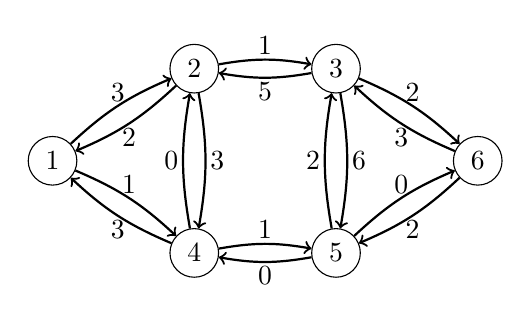
\begin{tikzpicture}[scale=0.9,label distance=-2mm]
\node[draw, circle] (1) at (1,1.3) {$1$};
\node[draw, circle] (2) at (3,2.6) {$2$};
\node[draw, circle] (3) at (5,2.6) {$3$};
\node[draw, circle] (4) at (7,1.3) {$6$};
\node[draw, circle] (5) at (3,0) {$4$};
\node[draw, circle] (6) at (5,0) {$5$};

\path[draw,thick,->] (1) edge [bend left=10] node[font=\small,label=3] {} (2);
\path[draw,thick,->] (2) edge [bend left=10] node[font=\small,label=below:2] {} (1);
\path[draw,thick,->] (2) edge [bend left=10] node[font=\small,label=1] {} (3);
\path[draw,thick,->] (3) edge [bend left=10] node[font=\small,label=below:5] {} (2);
\path[draw,thick,->] (3) edge [bend left=10] node[font=\small,label=2] {} (4);
\path[draw,thick,->] (4) edge [bend left=10] node[font=\small,label=below:3] {} (3);
\path[draw,thick,->] (1) edge [bend left=10] node[font=\small,label=1] {} (5);
\path[draw,thick,->] (5) edge [bend left=10] node[font=\small,label=below:3] {} (1);
\path[draw,thick,->] (5) edge [bend left=10] node[font=\small,label=1] {} (6);
\path[draw,thick,->] (6) edge [bend left=10] node[font=\small,label=below:0] {} (5);
\path[draw,thick,->] (6) edge [bend left=10] node[font=\small,label=0] {} (4);
\path[draw,thick,->] (4) edge [bend left=10] node[font=\small,label=below:2] {} (6);
\path[draw,thick,->] (5) edge [bend left=10] node[font=\small,label=left:0] {} (2);
\path[draw,thick,->] (2) edge [bend left=10] node[font=\small,label=right:3] {} (5);
\path[draw,thick,->] (3) edge [bend left=10] node[font=\small,label=right:6] {} (6);
\path[draw,thick,->] (6) edge [bend left=10] node[font=\small,label=left:2] {} (3);
\end{tikzpicture}
\end{center}
\end{samepage}

We still need two more rounds before reaching the maximum flow.
For example, we can choose the paths
$1 \rightarrow 2 \rightarrow 3 \rightarrow 6$ and
$1 \rightarrow 4 \rightarrow 5 \rightarrow 3 \rightarrow 6$.
Both paths increase the flow by 1,
and the final graph is as follows:

\begin{center}
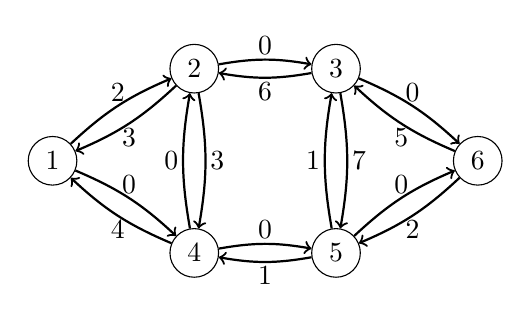
\begin{tikzpicture}[scale=0.9,label distance=-2mm]
\node[draw, circle] (1) at (1,1.3) {$1$};
\node[draw, circle] (2) at (3,2.6) {$2$};
\node[draw, circle] (3) at (5,2.6) {$3$};
\node[draw, circle] (4) at (7,1.3) {$6$};
\node[draw, circle] (5) at (3,0) {$4$};
\node[draw, circle] (6) at (5,0) {$5$};

\path[draw,thick,->] (1) edge [bend left=10] node[font=\small,label=2] {} (2);
\path[draw,thick,->] (2) edge [bend left=10] node[font=\small,label=below:3] {} (1);
\path[draw,thick,->] (2) edge [bend left=10] node[font=\small,label=0] {} (3);
\path[draw,thick,->] (3) edge [bend left=10] node[font=\small,label=below:6] {} (2);
\path[draw,thick,->] (3) edge [bend left=10] node[font=\small,label=0] {} (4);
\path[draw,thick,->] (4) edge [bend left=10] node[font=\small,label=below:5] {} (3);
\path[draw,thick,->] (1) edge [bend left=10] node[font=\small,label=0] {} (5);
\path[draw,thick,->] (5) edge [bend left=10] node[font=\small,label=below:4] {} (1);
\path[draw,thick,->] (5) edge [bend left=10] node[font=\small,label=0] {} (6);
\path[draw,thick,->] (6) edge [bend left=10] node[font=\small,label=below:1] {} (5);
\path[draw,thick,->] (6) edge [bend left=10] node[font=\small,label=0] {} (4);
\path[draw,thick,->] (4) edge [bend left=10] node[font=\small,label=below:2] {} (6);
\path[draw,thick,->] (5) edge [bend left=10] node[font=\small,label=left:0] {} (2);
\path[draw,thick,->] (2) edge [bend left=10] node[font=\small,label=right:3] {} (5);
\path[draw,thick,->] (3) edge [bend left=10] node[font=\small,label=right:7] {} (6);
\path[draw,thick,->] (6) edge [bend left=10] node[font=\small,label=left:1] {} (3);
\end{tikzpicture}
\end{center}

It is not possible to increase the flow anymore,
because there is no path from the source
to the sink with positive edge weights.
Hence, the algorithm terminates and the maximum flow is 7.

\subsubsection{Finding paths}

The Ford–Fulkerson algorithm does not specify
how we should choose the paths that increase the flow.
In any case, the algorithm will terminate sooner or later
and correctly find the maximum flow.
However, the efficiency of the algorithm depends on
the way the paths are chosen.

A simple way to find paths is to use depth-first search.
Usually, this works well, but in the worst case,
each path only increases the flow by 1
and the algorithm is slow.
Fortunately, we can avoid this situation
by using one of the following techniques:

\index{Edmonds–Karp algorithm}

The \key{Edmonds–Karp algorithm} \cite{edm72}
chooses each path so that the number of edges
on the path is as small as possible.
This can be done by using breadth-first search
instead of depth-first search for finding paths.
It can be proven that this guarantees that
the flow increases quickly, and the time complexity
of the algorithm is $O(m^2 n)$.

\index{scaling algorithm}

The \key{scaling algorithm} \cite{ahu91} uses depth-first
search to find paths where each edge weight is
at least a threshold value.
Initially, the threshold value is
some large number, for example the sum of all
edge weights of the graph.
Always when a path cannot be found,
the threshold value is divided by 2.
The time complexity of the algorithm is $O(m^2 \log c)$,
where $c$ is the initial threshold value.

In practice, the scaling algorithm is easier to implement,
because depth-first search can be used for finding paths.
Both algorithms are efficient enough for problems
that typically appear in programming contests.

\subsubsection{Minimum cuts}

\index{minimum cut}

It turns out that once the Ford–Fulkerson algorithm
has found a maximum flow,
it has also determined a minimum cut.
Let $A$ be the set of nodes
that can be reached from the source
using positive-weight edges, and $B$ the remaining nodes.
In the example graph, $A$ contains nodes 1, 2 and 4:

\begin{center}
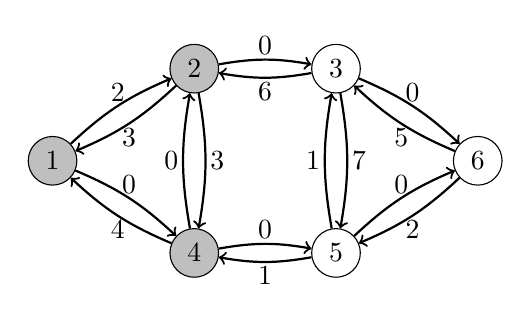
\begin{tikzpicture}[scale=0.9,label distance=-2mm]
\node[draw, circle,fill=lightgray] (1) at (1,1.3) {$1$};
\node[draw, circle,fill=lightgray] (2) at (3,2.6) {$2$};
\node[draw, circle] (3) at (5,2.6) {$3$};
\node[draw, circle] (4) at (7,1.3) {$6$};
\node[draw, circle,fill=lightgray] (5) at (3,0) {$4$};
\node[draw, circle] (6) at (5,0) {$5$};

\path[draw,thick,->] (1) edge [bend left=10] node[font=\small,label=2] {} (2);
\path[draw,thick,->] (2) edge [bend left=10] node[font=\small,label=below:3] {} (1);
\path[draw,thick,->] (2) edge [bend left=10] node[font=\small,label=0] {} (3);
\path[draw,thick,->] (3) edge [bend left=10] node[font=\small,label=below:6] {} (2);
\path[draw,thick,->] (3) edge [bend left=10] node[font=\small,label=0] {} (4);
\path[draw,thick,->] (4) edge [bend left=10] node[font=\small,label=below:5] {} (3);
\path[draw,thick,->] (1) edge [bend left=10] node[font=\small,label=0] {} (5);
\path[draw,thick,->] (5) edge [bend left=10] node[font=\small,label=below:4] {} (1);
\path[draw,thick,->] (5) edge [bend left=10] node[font=\small,label=0] {} (6);
\path[draw,thick,->] (6) edge [bend left=10] node[font=\small,label=below:1] {} (5);
\path[draw,thick,->] (6) edge [bend left=10] node[font=\small,label=0] {} (4);
\path[draw,thick,->] (4) edge [bend left=10] node[font=\small,label=below:2] {} (6);
\path[draw,thick,->] (5) edge [bend left=10] node[font=\small,label=left:0] {} (2);
\path[draw,thick,->] (2) edge [bend left=10] node[font=\small,label=right:3] {} (5);
\path[draw,thick,->] (3) edge [bend left=10] node[font=\small,label=right:7] {} (6);
\path[draw,thick,->] (6) edge [bend left=10] node[font=\small,label=left:1] {} (3);
\end{tikzpicture}
\end{center}

Now the minimum cut consists of the edges of the original graph
that start at some node in $A$, end at some node outside $A$,
and whose capacity is fully
used in the maximum flow.
In the above graph, such edges are
$2 \rightarrow 3$ and $4 \rightarrow 5$,
that correspond to the minimum cut $6+1=7$.

Why is the flow produced by the algorithm maximum
and why is the cut minimum?
The reason is that a graph cannot
contain a flow whose size is larger
than the weight of any cut of the graph.
Hence, always when a flow and a cut are equally large,
they are a maximum flow and a minimum cut.

Let us consider any cut of the graph
such that the source belongs to $A$,
the sink belongs to $B$
and there are some edges between the sets:

\begin{center}
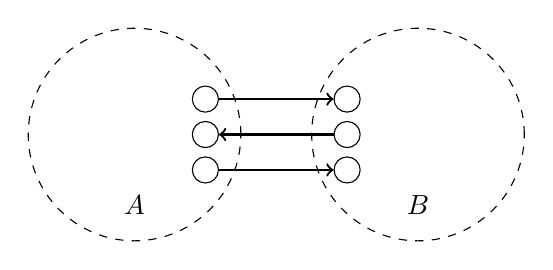
\begin{tikzpicture}[scale=0.9]
\draw[dashed] (-2,0) circle (1.5);
\draw[dashed] (2,0) circle (1.5);

\node at (-2,-1) {$A$};
\node at (2,-1) {$B$};

\node[draw, circle] (1) at (-1,0.5) {};
\node[draw, circle] (2) at (-1,0) {};
\node[draw, circle] (3) at (-1,-0.5) {};
\node[draw, circle] (4) at (1,0.5) {};
\node[draw, circle] (5) at (1,0) {};
\node[draw, circle] (6) at (1,-0.5) {};

\path[draw,thick,->] (1) -- (4);
\path[draw,thick,->] (5) -- (2);
\path[draw,thick,->] (3) -- (6);

\end{tikzpicture}
\end{center}

The size of the cut is the sum of the edges
that go from $A$ to $B$.
This is an upper bound for the flow
in the graph, because the flow has to proceed
from $A$ to $B$.
Thus, the size of a maximum flow is smaller than or equal to
the size of any cut in the graph.

On the other hand, the Ford–Fulkerson algorithm
produces a flow whose size is \emph{exactly} as large
as the size of a cut in the graph.
Thus, the flow has to be a maximum flow
and the cut has to be a minimum cut.

\section{Disjoint paths}

Many graph problems can be solved by reducing
them to the maximum flow problem.
Our first example of such a problem is
as follows: we are given a directed graph
with a source and a sink,
and our task is to find the maximum number
of disjoint paths from the source to the sink.

\subsubsection{Edge-disjoint paths}

We will first focus on the problem of
finding the maximum number of
\key{edge-disjoint paths} from the source to the sink.
This means that we should construct a set of paths
such that each edge appears in at most one path.

For example, consider the following graph:
\begin{center}
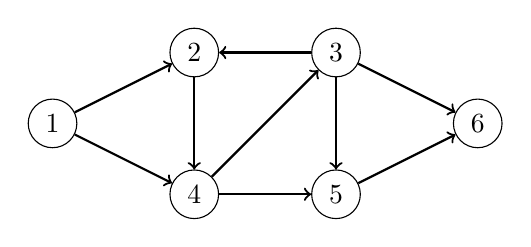
\begin{tikzpicture}[scale=0.9]
\node[draw, circle] (1) at (1,2) {$1$};
\node[draw, circle] (2) at (3,3) {$2$};
\node[draw, circle] (3) at (5,3) {$3$};
\node[draw, circle] (4) at (3,1) {$4$};
\node[draw, circle] (5) at (5,1) {$5$};
\node[draw, circle] (6) at (7,2) {$6$};
\path[draw,thick,->] (1) -- (2);
\path[draw,thick,->] (1) -- (4);
\path[draw,thick,->] (2) -- (4);
\path[draw,thick,->] (3) -- (2);
\path[draw,thick,->] (3) -- (5);
\path[draw,thick,->] (3) -- (6);
\path[draw,thick,->] (4) -- (3);
\path[draw,thick,->] (4) -- (5);
\path[draw,thick,->] (5) -- (6);
\end{tikzpicture}
\end{center}

In this graph, the maximum number of edge-disjoint
paths is 2.
We can choose the paths
$1 \rightarrow 2 \rightarrow 4 \rightarrow 3 \rightarrow 6$
and $1 \rightarrow 4 \rightarrow 5 \rightarrow 6$ as follows:

\begin{center}
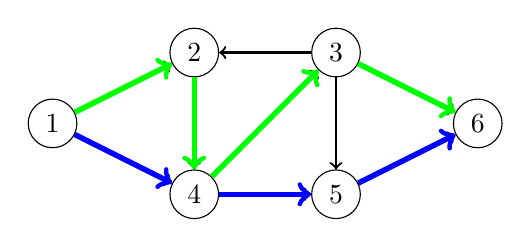
\begin{tikzpicture}[scale=0.9]
\node[draw, circle] (1) at (1,2) {$1$};
\node[draw, circle] (2) at (3,3) {$2$};
\node[draw, circle] (3) at (5,3) {$3$};
\node[draw, circle] (4) at (3,1) {$4$};
\node[draw, circle] (5) at (5,1) {$5$};
\node[draw, circle] (6) at (7,2) {$6$};
\path[draw,thick,->] (1) -- (2);
\path[draw,thick,->] (1) -- (4);
\path[draw,thick,->] (2) -- (4);
\path[draw,thick,->] (3) -- (2);
\path[draw,thick,->] (3) -- (5);
\path[draw,thick,->] (3) -- (6);
\path[draw,thick,->] (4) -- (3);
\path[draw,thick,->] (4) -- (5);
\path[draw,thick,->] (5) -- (6);

\path[draw=green,thick,->,line width=2pt] (1) -- (2);
\path[draw=green,thick,->,line width=2pt] (2) -- (4);
\path[draw=green,thick,->,line width=2pt] (4) -- (3);
\path[draw=green,thick,->,line width=2pt] (3) -- (6);

\path[draw=blue,thick,->,line width=2pt] (1) -- (4);
\path[draw=blue,thick,->,line width=2pt] (4) -- (5);
\path[draw=blue,thick,->,line width=2pt] (5) -- (6);
\end{tikzpicture}
\end{center}

It turns out that the maximum number of
edge-disjoint paths
equals the maximum flow of the graph,
assuming that the capacity of each edge is one.
After the maximum flow has been constructed,
the edge-disjoint paths can be found greedily
by following paths from the source to the sink.

\subsubsection{Node-disjoint paths}

Let us now consider another problem:
finding the maximum number of
\key{node-disjoint paths} from the source
to the sink.
In this problem, every node,
except for the source and sink,
may appear in at most one path.
The number of node-disjoint paths
may be smaller than the number of
edge-disjoint paths.

For example, in the previous graph,
the maximum number of node-disjoint paths is 1:

\begin{center}
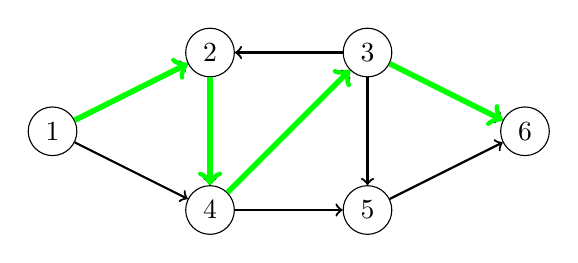
\begin{tikzpicture}
\node[draw, circle] (1) at (1,2) {$1$};
\node[draw, circle] (2) at (3,3) {$2$};
\node[draw, circle] (3) at (5,3) {$3$};
\node[draw, circle] (4) at (3,1) {$4$};
\node[draw, circle] (5) at (5,1) {$5$};
\node[draw, circle] (6) at (7,2) {$6$};
\path[draw,thick,->] (1) -- (2);
\path[draw,thick,->] (1) -- (4);
\path[draw,thick,->] (2) -- (4);
\path[draw,thick,->] (3) -- (2);
\path[draw,thick,->] (3) -- (5);
\path[draw,thick,->] (3) -- (6);
\path[draw,thick,->] (4) -- (3);
\path[draw,thick,->] (4) -- (5);
\path[draw,thick,->] (5) -- (6);

\path[draw=green,thick,->,line width=2pt] (1) -- (2);
\path[draw=green,thick,->,line width=2pt] (2) -- (4);
\path[draw=green,thick,->,line width=2pt] (4) -- (3);
\path[draw=green,thick,->,line width=2pt] (3) -- (6);
\end{tikzpicture}
\end{center}

We can reduce also this problem to the maximum flow problem.
Since each node can appear in at most one path,
we have to limit the flow that goes through the nodes.
A standard method for this is to divide each node into
two nodes such that the first node has the incoming edges
of the original node, the second node has the outgoing
edges of the original node, and
there is a new edge from the first node
to the second node.

In our example, the graph becomes as follows:
\begin{center}
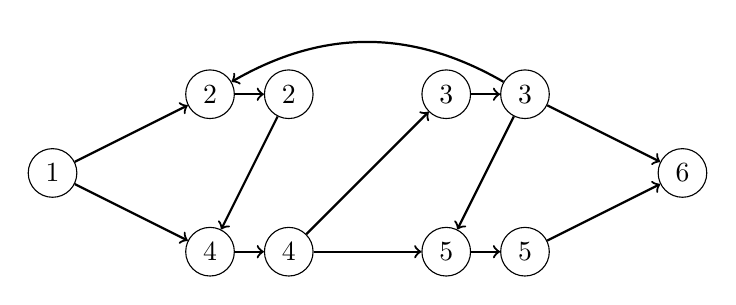
\begin{tikzpicture}
\node[draw, circle] (1) at (1,2) {$1$};

\node[draw, circle] (2a) at (3,3) {$2$};
\node[draw, circle] (3a) at (6,3) {$3$};
\node[draw, circle] (4a) at (3,1) {$4$};
\node[draw, circle] (5a) at (6,1) {$5$};

\node[draw, circle] (2b) at (4,3) {$2$};
\node[draw, circle] (3b) at (7,3) {$3$};
\node[draw, circle] (4b) at (4,1) {$4$};
\node[draw, circle] (5b) at (7,1) {$5$};

\node[draw, circle] (6) at (9,2) {$6$};

\path[draw,thick,->] (2a) -- (2b);
\path[draw,thick,->] (3a) -- (3b);
\path[draw,thick,->] (4a) -- (4b);
\path[draw,thick,->] (5a) -- (5b);

\path[draw,thick,->] (1) -- (2a);
\path[draw,thick,->] (1) -- (4a);
\path[draw,thick,->] (2b) -- (4a);
\path[draw,thick,->] (3b) edge [bend right=30] (2a);
\path[draw,thick,->] (3b) -- (5a);
\path[draw,thick,->] (3b) -- (6);
\path[draw,thick,->] (4b) -- (3a);
\path[draw,thick,->] (4b) -- (5a);
\path[draw,thick,->] (5b) -- (6);
\end{tikzpicture}
\end{center}

The maximum flow for the graph is as follows:
\begin{center}
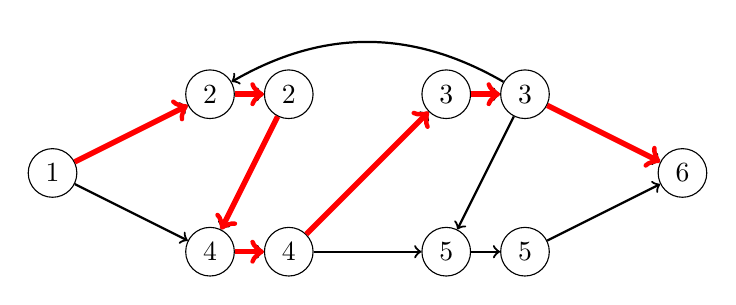
\begin{tikzpicture}
\node[draw, circle] (1) at (1,2) {$1$};

\node[draw, circle] (2a) at (3,3) {$2$};
\node[draw, circle] (3a) at (6,3) {$3$};
\node[draw, circle] (4a) at (3,1) {$4$};
\node[draw, circle] (5a) at (6,1) {$5$};

\node[draw, circle] (2b) at (4,3) {$2$};
\node[draw, circle] (3b) at (7,3) {$3$};
\node[draw, circle] (4b) at (4,1) {$4$};
\node[draw, circle] (5b) at (7,1) {$5$};

\node[draw, circle] (6) at (9,2) {$6$};

\path[draw,thick,->] (2a) -- (2b);
\path[draw,thick,->] (3a) -- (3b);
\path[draw,thick,->] (4a) -- (4b);
\path[draw,thick,->] (5a) -- (5b);

\path[draw,thick,->] (1) -- (2a);
\path[draw,thick,->] (1) -- (4a);
\path[draw,thick,->] (2b) -- (4a);
\path[draw,thick,->] (3b) edge [bend right=30] (2a);
\path[draw,thick,->] (3b) -- (5a);
\path[draw,thick,->] (3b) -- (6);
\path[draw,thick,->] (4b) -- (3a);
\path[draw,thick,->] (4b) -- (5a);
\path[draw,thick,->] (5b) -- (6);

\path[draw=red,thick,->,line width=2pt] (1) -- (2a);
\path[draw=red,thick,->,line width=2pt] (2a) -- (2b);
\path[draw=red,thick,->,line width=2pt] (2b) -- (4a);
\path[draw=red,thick,->,line width=2pt] (4a) -- (4b);
\path[draw=red,thick,->,line width=2pt] (4b) -- (3a);
\path[draw=red,thick,->,line width=2pt] (3a) -- (3b);
\path[draw=red,thick,->,line width=2pt] (3b) -- (6);
\end{tikzpicture}
\end{center}

Thus, the maximum number of node-disjoint paths
from the source to the sink is 1.

\section{Maximum matchings}

\index{matching}
\index{maximum matching}

The \key{maximum matching} problem asks to find
a maximum-size set of node pairs in an undirected graph
such that each pair is connected with an edge and
each node belongs to at most one pair.

There are polynomial algorithms for finding
maximum matchings in general graphs \cite{edm65},
but such algorithms are complex and
rarely seen in programming contests.
However, in bipartite graphs,
the maximum matching problem is much easier
to solve, because we can reduce it to the
maximum flow problem.

\subsubsection{Finding maximum matchings}

The nodes of a bipartite graph can be always
divided into two groups such that all edges
of the graph go from the left group to the right group.
For example, in the following bipartite graph,
the groups are $\{1,2,3,4\}$ and $\{5,6,7,8\}$.

\begin{center}
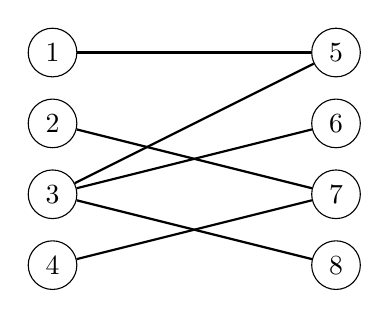
\begin{tikzpicture}[scale=0.60]
\node[draw, circle] (1) at (2,4.5) {1};
\node[draw, circle] (2) at (2,3) {2};
\node[draw, circle] (3) at (2,1.5) {3};
\node[draw, circle] (4) at (2,0) {4};
\node[draw, circle] (5) at (8,4.5) {5};
\node[draw, circle] (6) at (8,3) {6};
\node[draw, circle] (7) at (8,1.5) {7};
\node[draw, circle] (8) at (8,0) {8};

\path[draw,thick,-] (1) -- (5);
\path[draw,thick,-] (2) -- (7);
\path[draw,thick,-] (3) -- (5);
\path[draw,thick,-] (3) -- (6);
\path[draw,thick,-] (3) -- (8);
\path[draw,thick,-] (4) -- (7);
\end{tikzpicture}
\end{center}
The size of a maximum matching of this graph is 3:
\begin{center}
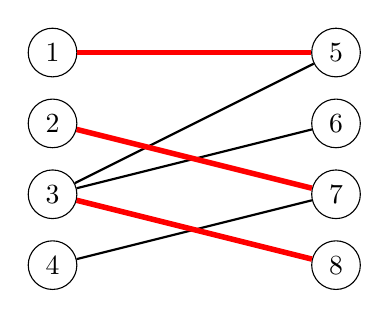
\begin{tikzpicture}[scale=0.60]
\node[draw, circle] (1) at (2,4.5) {1};
\node[draw, circle] (2) at (2,3) {2};
\node[draw, circle] (3) at (2,1.5) {3};
\node[draw, circle] (4) at (2,0) {4};
\node[draw, circle] (5) at (8,4.5) {5};
\node[draw, circle] (6) at (8,3) {6};
\node[draw, circle] (7) at (8,1.5) {7};
\node[draw, circle] (8) at (8,0) {8};

\path[draw,thick,-] (1) -- (5);
\path[draw,thick,-] (2) -- (7);
\path[draw,thick,-] (3) -- (5);
\path[draw,thick,-] (3) -- (6);
\path[draw,thick,-] (3) -- (8);
\path[draw,thick,-] (4) -- (7);

\path[draw=red,thick,-,line width=2pt] (1) -- (5);
\path[draw=red,thick,-,line width=2pt] (2) -- (7);
\path[draw=red,thick,-,line width=2pt] (3) -- (8);
\end{tikzpicture}
\end{center}

We can reduce the bipartite maximum matching problem
to the maximum flow problem by adding two new nodes
to the graph: a source and a sink.
We also add edges from the source
to each left node and from each right node to the sink.
After this, the size of a maximum flow in the graph
equals the size of a maximum matching in the original graph.

For example, the reduction for the above
graph is as follows:
\begin{center}
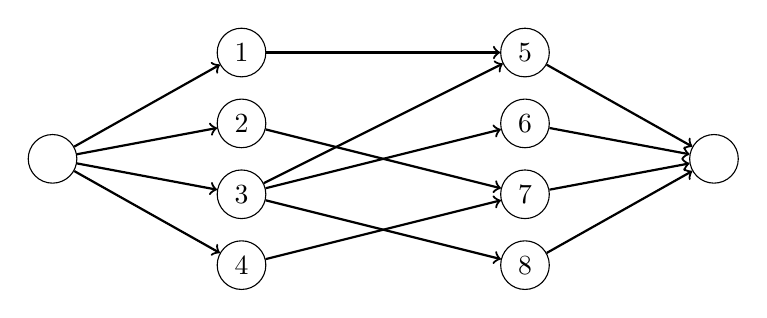
\begin{tikzpicture}[scale=0.60]
\node[draw, circle] (1) at (2,4.5) {1};
\node[draw, circle] (2) at (2,3) {2};
\node[draw, circle] (3) at (2,1.5) {3};
\node[draw, circle] (4) at (2,0) {4};
\node[draw, circle] (5) at (8,4.5) {5};
\node[draw, circle] (6) at (8,3) {6};
\node[draw, circle] (7) at (8,1.5) {7};
\node[draw, circle] (8) at (8,0) {8};

\node[draw, circle] (a) at (-2,2.25) {\phantom{0}};
\node[draw, circle] (b) at (12,2.25) {\phantom{0}};

\path[draw,thick,->] (1) -- (5);
\path[draw,thick,->] (2) -- (7);
\path[draw,thick,->] (3) -- (5);
\path[draw,thick,->] (3) -- (6);
\path[draw,thick,->] (3) -- (8);
\path[draw,thick,->] (4) -- (7);

\path[draw,thick,->] (a) -- (1);
\path[draw,thick,->] (a) -- (2);
\path[draw,thick,->] (a) -- (3);
\path[draw,thick,->] (a) -- (4);
\path[draw,thick,->] (5) -- (b);
\path[draw,thick,->] (6) -- (b);
\path[draw,thick,->] (7) -- (b);
\path[draw,thick,->] (8) -- (b);
\end{tikzpicture}
\end{center}

The maximum flow of this graph is as follows:
\begin{center}
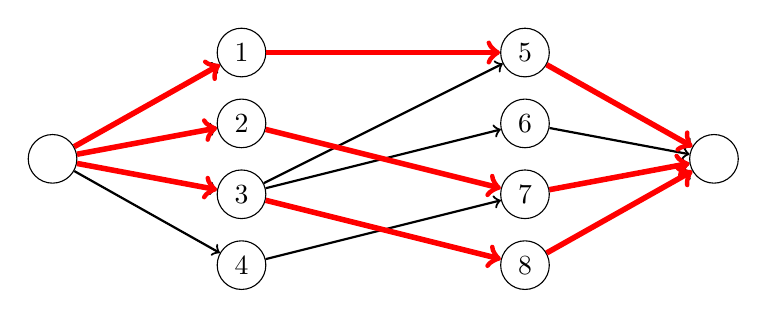
\begin{tikzpicture}[scale=0.60]
\node[draw, circle] (1) at (2,4.5) {1};
\node[draw, circle] (2) at (2,3) {2};
\node[draw, circle] (3) at (2,1.5) {3};
\node[draw, circle] (4) at (2,0) {4};
\node[draw, circle] (5) at (8,4.5) {5};
\node[draw, circle] (6) at (8,3) {6};
\node[draw, circle] (7) at (8,1.5) {7};
\node[draw, circle] (8) at (8,0) {8};

\node[draw, circle] (a) at (-2,2.25) {\phantom{0}};
\node[draw, circle] (b) at (12,2.25) {\phantom{0}};

\path[draw,thick,->] (3) -- (5);
\path[draw,thick,->] (3) -- (6);
\path[draw,thick,->] (4) -- (7);

\path[draw,thick,->] (a) -- (1);
\path[draw,thick,->] (a) -- (2);
\path[draw,thick,->] (a) -- (3);
\path[draw,thick,->] (a) -- (4);
\path[draw,thick,->] (5) -- (b);
\path[draw,thick,->] (6) -- (b);
\path[draw,thick,->] (7) -- (b);
\path[draw,thick,->] (8) -- (b);

\path[draw=red,thick,->,line width=2pt] (1) -- (5);
\path[draw=red,thick,->,line width=2pt] (2) -- (7);
\path[draw=red,thick,->,line width=2pt] (3) -- (8);

\path[draw=red,thick,->,line width=2pt] (a) -- (1);
\path[draw=red,thick,->,line width=2pt] (a) -- (2);
\path[draw=red,thick,->,line width=2pt] (a) -- (3);

\path[draw=red,thick,->,line width=2pt] (5) -- (b);
\path[draw=red,thick,->,line width=2pt] (7) -- (b);
\path[draw=red,thick,->,line width=2pt] (8) -- (b);

\end{tikzpicture}
\end{center}

\subsubsection{Hall's theorem}

\index{Hall's theorem}
\index{perfect matching}

\key{Hall's theorem} can be used to find out
whether a bipartite graph has a matching
that contains all left or right nodes.
If the number of left and right nodes is the same,
Hall's theorem tells us if it is possible to
construct a \key{perfect matching} that
contains all nodes of the graph.

Assume that we want to find a matching
that contains all left nodes.
Let $X$ be any set of left nodes
and let $f(X)$ be the set of their neighbors.
According to Hall's theorem, a matching
that contains all left nodes exists
exactly when for each $X$, the condition $|X| \le |f(X)|$ holds.

Let us study Hall's theorem in the example graph.
First, let $X=\{1,3\}$ which yields $f(X)=\{5,6,8\}$:

\begin{center}
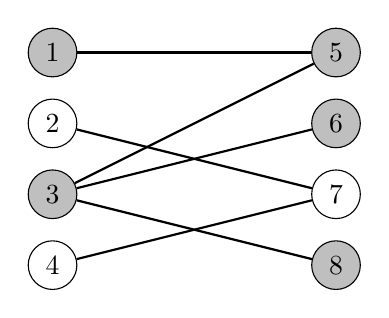
\begin{tikzpicture}[scale=0.60]
\node[draw, circle, fill=lightgray] (1) at (2,4.5) {1};
\node[draw, circle] (2) at (2,3) {2};
\node[draw, circle, fill=lightgray] (3) at (2,1.5) {3};
\node[draw, circle] (4) at (2,0) {4};
\node[draw, circle, fill=lightgray] (5) at (8,4.5) {5};
\node[draw, circle, fill=lightgray] (6) at (8,3) {6};
\node[draw, circle] (7) at (8,1.5) {7};
\node[draw, circle, fill=lightgray] (8) at (8,0) {8};

\path[draw,thick,-] (1) -- (5);
\path[draw,thick,-] (2) -- (7);
\path[draw,thick,-] (3) -- (5);
\path[draw,thick,-] (3) -- (6);
\path[draw,thick,-] (3) -- (8);
\path[draw,thick,-] (4) -- (7);
\end{tikzpicture}
\end{center}

The condition of Hall's theorem holds, because
$|X|=2$ and $|f(X)|=3$.
Next, let $X=\{2,4\}$ which yields $f(X)=\{7\}$:

\begin{center}
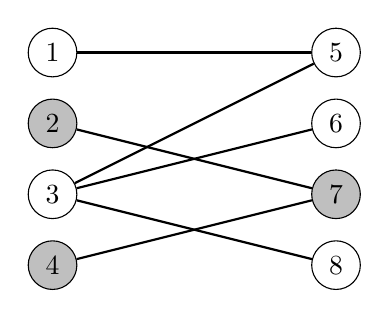
\begin{tikzpicture}[scale=0.60]
\node[draw, circle] (1) at (2,4.5) {1};
\node[draw, circle, fill=lightgray] (2) at (2,3) {2};
\node[draw, circle] (3) at (2,1.5) {3};
\node[draw, circle, fill=lightgray] (4) at (2,0) {4};
\node[draw, circle] (5) at (8,4.5) {5};
\node[draw, circle] (6) at (8,3) {6};
\node[draw, circle, fill=lightgray] (7) at (8,1.5) {7};
\node[draw, circle] (8) at (8,0) {8};

\path[draw,thick,-] (1) -- (5);
\path[draw,thick,-] (2) -- (7);
\path[draw,thick,-] (3) -- (5);
\path[draw,thick,-] (3) -- (6);
\path[draw,thick,-] (3) -- (8);
\path[draw,thick,-] (4) -- (7);
\end{tikzpicture}
\end{center}

In this case, $|X|=2$ and $|f(X)|=1$,
so the condition of Hall's theorem does not hold.
This means that it is not possible to form
a perfect matching for the graph.
This result is not surprising, because we already
know that the maximum matching of the graph is 3 and not 4.

If the condition of Hall's theorem does not hold,
the set $X$ provides an explanation \emph{why}
we cannot form such a matching.
Since $X$ contains more nodes than $f(X)$,
there are no pairs for all nodes in $X$.
For example, in the above graph, both nodes 2 and 4
should be connected with node 7 which is not possible.

\subsubsection{Kőnig's theorem}

\index{Kőnig's theorem}
\index{node cover}
\index{minimum node cover}

A \key{minimum node cover} of a graph
is a minimum set of nodes such that each edge of the graph
has at least one endpoint in the set.
In a general graph, finding a minimum node cover
is a NP-hard problem.
However, if the graph is bipartite,
\key{Kőnig's theorem} tells us that
the size of a minimum node cover
and the size of a maximum matching are always equal.
Thus, we can calculate the size of a minimum node cover
using a maximum flow algorithm.

Let us consider the following graph
with a maximum matching of size 3:
\begin{center}
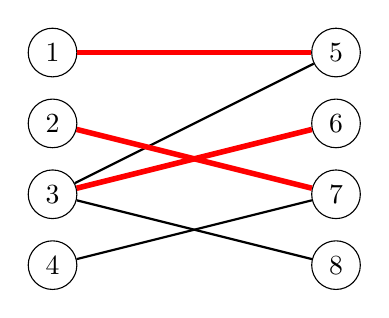
\begin{tikzpicture}[scale=0.60]
\node[draw, circle] (1) at (2,4.5) {1};
\node[draw, circle] (2) at (2,3) {2};
\node[draw, circle] (3) at (2,1.5) {3};
\node[draw, circle] (4) at (2,0) {4};
\node[draw, circle] (5) at (8,4.5) {5};
\node[draw, circle] (6) at (8,3) {6};
\node[draw, circle] (7) at (8,1.5) {7};
\node[draw, circle] (8) at (8,0) {8};

\path[draw,thick,-] (1) -- (5);
\path[draw,thick,-] (2) -- (7);
\path[draw,thick,-] (3) -- (5);
\path[draw,thick,-] (3) -- (6);
\path[draw,thick,-] (3) -- (8);
\path[draw,thick,-] (4) -- (7);

\path[draw=red,thick,-,line width=2pt] (1) -- (5);
\path[draw=red,thick,-,line width=2pt] (2) -- (7);
\path[draw=red,thick,-,line width=2pt] (3) -- (6);
\end{tikzpicture}
\end{center}
Now Kőnig's theorem tells us that the size
of a minimum node cover is also 3.
Such a cover can be constructed as follows:

\begin{center}
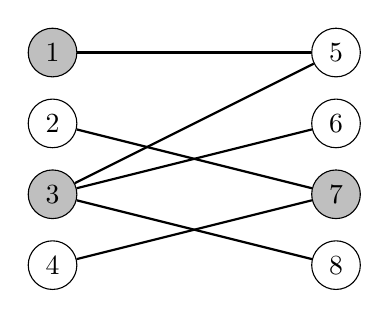
\begin{tikzpicture}[scale=0.60]
\node[draw, circle, fill=lightgray] (1) at (2,4.5) {1};
\node[draw, circle] (2) at (2,3) {2};
\node[draw, circle, fill=lightgray] (3) at (2,1.5) {3};
\node[draw, circle] (4) at (2,0) {4};
\node[draw, circle] (5) at (8,4.5) {5};
\node[draw, circle] (6) at (8,3) {6};
\node[draw, circle, fill=lightgray] (7) at (8,1.5) {7};
\node[draw, circle] (8) at (8,0) {8};

\path[draw,thick,-] (1) -- (5);
\path[draw,thick,-] (2) -- (7);
\path[draw,thick,-] (3) -- (5);
\path[draw,thick,-] (3) -- (6);
\path[draw,thick,-] (3) -- (8);
\path[draw,thick,-] (4) -- (7);
\end{tikzpicture}
\end{center}

\index{independent set}
\index{maximum independent set}

The nodes that do \emph{not}
belong to a minimum node cover
form a \key{maximum independent set}.
This is the largest possible set of nodes
such that no two nodes in the set
are connected with an edge.
Once again, finding a maximum independent
set in a general graph is a NP-hard problem,
but in a bipartite graph we can use
Kőnig's theorem to solve the problem efficiently.
In the example graph, the maximum independent
set is as follows:

\begin{center}
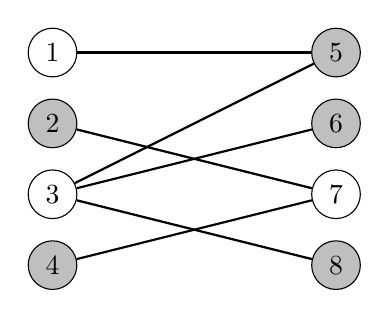
\begin{tikzpicture}[scale=0.60]
\node[draw, circle] (1) at (2,4.5) {1};
\node[draw, circle, fill=lightgray] (2) at (2,3) {2};
\node[draw, circle] (3) at (2,1.5) {3};
\node[draw, circle, fill=lightgray] (4) at (2,0) {4};
\node[draw, circle, fill=lightgray] (5) at (8,4.5) {5};
\node[draw, circle, fill=lightgray] (6) at (8,3) {6};
\node[draw, circle] (7) at (8,1.5) {7};
\node[draw, circle, fill=lightgray] (8) at (8,0) {8};

\path[draw,thick,-] (1) -- (5);
\path[draw,thick,-] (2) -- (7);
\path[draw,thick,-] (3) -- (5);
\path[draw,thick,-] (3) -- (6);
\path[draw,thick,-] (3) -- (8);
\path[draw,thick,-] (4) -- (7);
\end{tikzpicture}
\end{center}

\section{Path covers}

\index{path cover}

A \key{path cover} is a set of paths in a graph
such that each node of the graph belongs to at least one path.
It turns out that in directed, acyclic graphs,
we can reduce the problem of finding a minimum
path cover to the problem of finding a maximum
flow in another graph.

\subsubsection{Node-disjoint path cover}

In a \key{node-disjoint path cover},
each node belongs to exactly one path.
As an example, consider the following graph:
\begin{center}
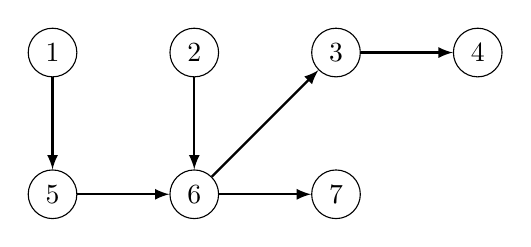
\begin{tikzpicture}[scale=0.9]
\node[draw, circle] (1) at (0,0) {1};
\node[draw, circle] (2) at (2,0) {2};
\node[draw, circle] (3) at (4,0) {3};
\node[draw, circle] (4) at (6,0) {4};
\node[draw, circle] (5) at (0,-2) {5};
\node[draw, circle] (6) at (2,-2) {6};
\node[draw, circle] (7) at (4,-2) {7};

\path[draw,thick,->,>=latex] (1) -- (5);
\path[draw,thick,->,>=latex] (2) -- (6);
\path[draw,thick,->,>=latex] (3) -- (4);
\path[draw,thick,->,>=latex] (5) -- (6);
\path[draw,thick,->,>=latex] (6) -- (3);
\path[draw,thick,->,>=latex] (6) -- (7);
\end{tikzpicture}
\end{center}

A minimum node-disjoint path cover
of this graph
consists of three paths.
For example, we can choose the following paths:

\begin{center}
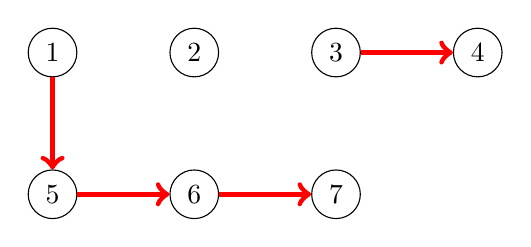
\begin{tikzpicture}[scale=0.9]
\node[draw, circle] (1) at (0,0) {1};
\node[draw, circle] (2) at (2,0) {2};
\node[draw, circle] (3) at (4,0) {3};
\node[draw, circle] (4) at (6,0) {4};
\node[draw, circle] (5) at (0,-2) {5};
\node[draw, circle] (6) at (2,-2) {6};
\node[draw, circle] (7) at (4,-2) {7};

\path[draw=red,thick,->,line width=2pt] (1) -- (5);
\path[draw=red,thick,->,line width=2pt] (5) -- (6);
\path[draw=red,thick,->,line width=2pt] (6) -- (7);
\path[draw=red,thick,->,line width=2pt] (3) -- (4);
\end{tikzpicture}
\end{center}

Note that one of the paths only contains node 2,
so it is possible that a path does not contain any edges.

We can find a minimum node-disjoint path cover
by constructing a \emph{matching graph} where each node
of the original graph is represented by
two nodes: a left node and a right node.
There is an edge from a left node to a right node
if there is such an edge in the original graph.
In addition, the matching graph contains a source and a sink,
and there are edges from the source to all
left nodes and from all right nodes to the sink.

A maximum matching in the resulting graph corresponds
to a minimum node-disjoint path cover in
the original graph.
For example, the following matching graph
for the above graph contains
a maximum matching of size 4:

\begin{center}
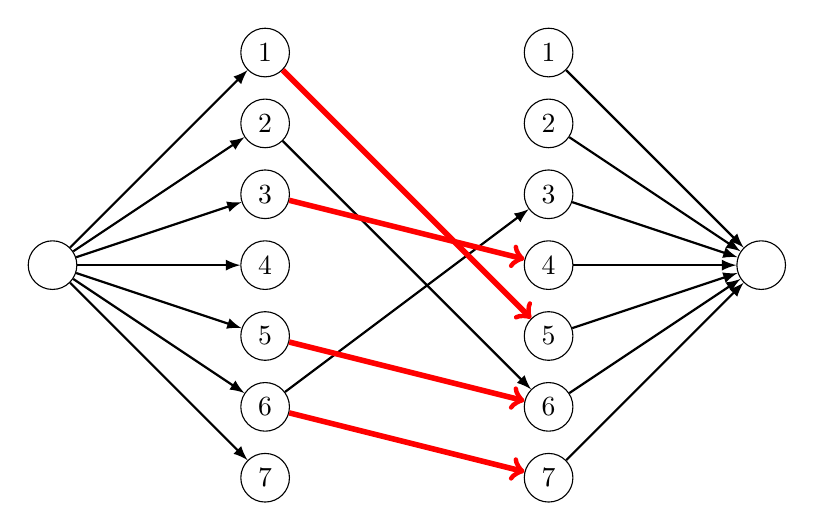
\begin{tikzpicture}[scale=0.9]
\node[draw, circle] (1a) at (0,6) {1};
\node[draw, circle] (2a) at (0,5) {2};
\node[draw, circle] (3a) at (0,4) {3};
\node[draw, circle] (4a) at (0,3) {4};
\node[draw, circle] (5a) at (0,2) {5};
\node[draw, circle] (6a) at (0,1) {6};
\node[draw, circle] (7a) at (0,0) {7};

\node[draw, circle] (1b) at (4,6) {1};
\node[draw, circle] (2b) at (4,5) {2};
\node[draw, circle] (3b) at (4,4) {3};
\node[draw, circle] (4b) at (4,3) {4};
\node[draw, circle] (5b) at (4,2) {5};
\node[draw, circle] (6b) at (4,1) {6};
\node[draw, circle] (7b) at (4,0) {7};

\node[draw, circle] (a) at (-3,3) {\phantom{0}};
\node[draw, circle] (b) at (7,3) {\phantom{0}};

%\path[draw,thick,->,>=latex] (1a) -- (5b);
\path[draw,thick,->,>=latex] (2a) -- (6b);
%\path[draw,thick,->,>=latex] (3a) -- (4b);
%\path[draw,thick,->,>=latex] (5a) -- (6b);
\path[draw,thick,->,>=latex] (6a) -- (3b);
%\path[draw,thick,->,>=latex] (6a) -- (7b);

\path[draw,thick,->,>=latex] (a) -- (1a);
\path[draw,thick,->,>=latex] (a) -- (2a);
\path[draw,thick,->,>=latex] (a) -- (3a);
\path[draw,thick,->,>=latex] (a) -- (4a);
\path[draw,thick,->,>=latex] (a) -- (5a);
\path[draw,thick,->,>=latex] (a) -- (6a);
\path[draw,thick,->,>=latex] (a) -- (7a);

\path[draw,thick,->,>=latex] (1b) -- (b);
\path[draw,thick,->,>=latex] (2b) -- (b);
\path[draw,thick,->,>=latex] (3b) -- (b);
\path[draw,thick,->,>=latex] (4b) -- (b);
\path[draw,thick,->,>=latex] (5b) -- (b);
\path[draw,thick,->,>=latex] (6b) -- (b);
\path[draw,thick,->,>=latex] (7b) -- (b);

\path[draw=red,thick,->,line width=2pt] (1a) -- (5b);
\path[draw=red,thick,->,line width=2pt] (5a) -- (6b);
\path[draw=red,thick,->,line width=2pt] (6a) -- (7b);
\path[draw=red,thick,->,line width=2pt] (3a) -- (4b);

\end{tikzpicture}
\end{center}

Each edge in the maximum matching of the matching graph corresponds
to an edge in the minimum node-disjoint path cover
of the original graph.
Thus, the size of the minimum node-disjoint path cover is $n-c$,
where $n$ is the number of nodes in the original graph
and $c$ is the size of the maximum matching.

\subsubsection{General path cover}

A \key{general path cover} is a path cover
where a node can belong to more than one path.
A minimum general path cover may be smaller
than a minimum node-disjoint path cover,
because a node can be used multiple times in paths.
Consider again the following graph:
\begin{center}
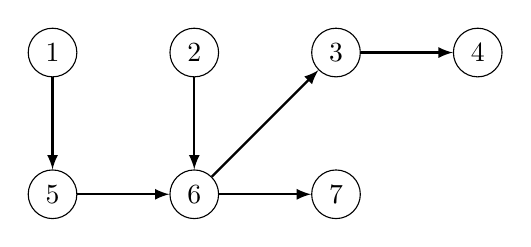
\begin{tikzpicture}[scale=0.9]
\node[draw, circle] (1) at (0,0) {1};
\node[draw, circle] (2) at (2,0) {2};
\node[draw, circle] (3) at (4,0) {3};
\node[draw, circle] (4) at (6,0) {4};
\node[draw, circle] (5) at (0,-2) {5};
\node[draw, circle] (6) at (2,-2) {6};
\node[draw, circle] (7) at (4,-2) {7};

\path[draw,thick,->,>=latex] (1) -- (5);
\path[draw,thick,->,>=latex] (2) -- (6);
\path[draw,thick,->,>=latex] (3) -- (4);
\path[draw,thick,->,>=latex] (5) -- (6);
\path[draw,thick,->,>=latex] (6) -- (3);
\path[draw,thick,->,>=latex] (6) -- (7);
\end{tikzpicture}
\end{center}

The minimum general path cover of this graph
consists of two paths.
For example, the first path may be as follows:
\begin{center}
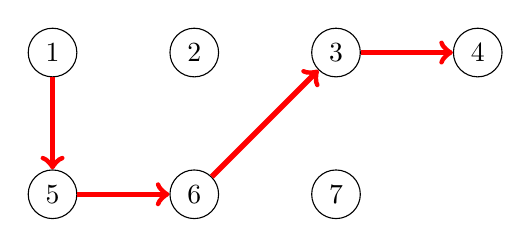
\begin{tikzpicture}[scale=0.9]
\node[draw, circle] (1) at (0,0) {1};
\node[draw, circle] (2) at (2,0) {2};
\node[draw, circle] (3) at (4,0) {3};
\node[draw, circle] (4) at (6,0) {4};
\node[draw, circle] (5) at (0,-2) {5};
\node[draw, circle] (6) at (2,-2) {6};
\node[draw, circle] (7) at (4,-2) {7};

\path[draw=red,thick,->,line width=2pt] (1) -- (5);
\path[draw=red,thick,->,line width=2pt] (5) -- (6);
\path[draw=red,thick,->,line width=2pt] (6) -- (3);
\path[draw=red,thick,->,line width=2pt] (3) -- (4);
\end{tikzpicture}
\end{center}
And the second path may be as follows:
\begin{center}
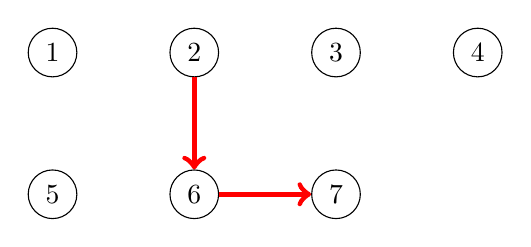
\begin{tikzpicture}[scale=0.9]
\node[draw, circle] (1) at (0,0) {1};
\node[draw, circle] (2) at (2,0) {2};
\node[draw, circle] (3) at (4,0) {3};
\node[draw, circle] (4) at (6,0) {4};
\node[draw, circle] (5) at (0,-2) {5};
\node[draw, circle] (6) at (2,-2) {6};
\node[draw, circle] (7) at (4,-2) {7};

\path[draw=red,thick,->,line width=2pt] (2) -- (6);
\path[draw=red,thick,->,line width=2pt] (6) -- (7);
\end{tikzpicture}
\end{center}

A minimum general path cover can be found
almost like a minimum node-disjoint path cover.
It suffices to add some new edges to the matching graph
so that there is an edge $a \rightarrow b$
always when there is a path from $a$ to $b$
in the original graph (possibly through several edges).

The matching graph for the above graph is as follows:
\begin{center}
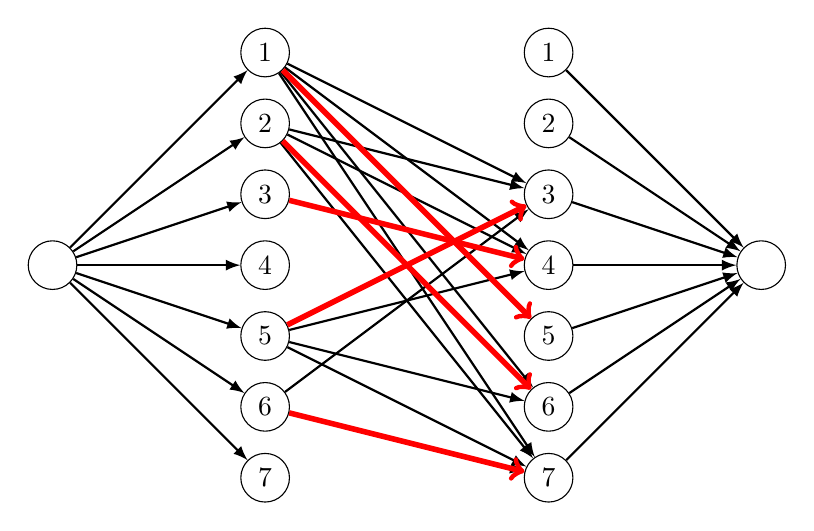
\begin{tikzpicture}[scale=0.9]
\node[draw, circle] (1a) at (0,6) {1};
\node[draw, circle] (2a) at (0,5) {2};
\node[draw, circle] (3a) at (0,4) {3};
\node[draw, circle] (4a) at (0,3) {4};
\node[draw, circle] (5a) at (0,2) {5};
\node[draw, circle] (6a) at (0,1) {6};
\node[draw, circle] (7a) at (0,0) {7};

\node[draw, circle] (1b) at (4,6) {1};
\node[draw, circle] (2b) at (4,5) {2};
\node[draw, circle] (3b) at (4,4) {3};
\node[draw, circle] (4b) at (4,3) {4};
\node[draw, circle] (5b) at (4,2) {5};
\node[draw, circle] (6b) at (4,1) {6};
\node[draw, circle] (7b) at (4,0) {7};

\node[draw, circle] (a) at (-3,3) {\phantom{0}};
\node[draw, circle] (b) at (7,3) {\phantom{0}};


%\path[draw,thick,->,>=latex] (1a) -- (5b);
\path[draw,thick,->,>=latex] (1a) -- (6b);
\path[draw,thick,->,>=latex] (1a) -- (7b);
\path[draw,thick,->,>=latex] (1a) -- (3b);
\path[draw,thick,->,>=latex] (1a) -- (4b);
\path[draw,thick,->,>=latex] (5a) -- (6b);
\path[draw,thick,->,>=latex] (5a) -- (7b);
%\path[draw,thick,->,>=latex] (5a) -- (3b);
\path[draw,thick,->,>=latex] (5a) -- (4b);
\path[draw,thick,->,>=latex] (6a) -- (7b);
%\path[draw,thick,->,>=latex] (6a) -- (7b);
\path[draw,thick,->,>=latex] (6a) -- (3b);
%\path[draw,thick,->,>=latex] (3a) -- (4b);
%\path[draw,thick,->,>=latex] (2a) -- (6b);
\path[draw,thick,->,>=latex] (2a) -- (7b);
\path[draw,thick,->,>=latex] (2a) -- (3b);
\path[draw,thick,->,>=latex] (2a) -- (4b);


\path[draw,thick,->,>=latex] (a) -- (1a);
\path[draw,thick,->,>=latex] (a) -- (2a);
\path[draw,thick,->,>=latex] (a) -- (3a);
\path[draw,thick,->,>=latex] (a) -- (4a);
\path[draw,thick,->,>=latex] (a) -- (5a);
\path[draw,thick,->,>=latex] (a) -- (6a);
\path[draw,thick,->,>=latex] (a) -- (7a);

\path[draw,thick,->,>=latex] (1b) -- (b);
\path[draw,thick,->,>=latex] (2b) -- (b);
\path[draw,thick,->,>=latex] (3b) -- (b);
\path[draw,thick,->,>=latex] (4b) -- (b);
\path[draw,thick,->,>=latex] (5b) -- (b);
\path[draw,thick,->,>=latex] (6b) -- (b);
\path[draw,thick,->,>=latex] (7b) -- (b);

\path[draw=red,thick,->,line width=2pt] (1a) -- (5b);
\path[draw=red,thick,->,line width=2pt] (5a) -- (3b);
\path[draw=red,thick,->,line width=2pt] (3a) -- (4b);
\path[draw=red,thick,->,line width=2pt] (2a) -- (6b);
\path[draw=red,thick,->,line width=2pt] (6a) -- (7b);


% \path[draw=red,thick,->,line width=2pt] (1a) -- (6b);
% \path[draw=red,thick,->,line width=2pt] (1a) -- (7b);
% \path[draw=red,thick,->,line width=2pt] (1a) -- (3b);
% \path[draw=red,thick,->,line width=2pt] (1a) -- (4b);
% \path[draw=red,thick,->,line width=2pt] (5a) -- (6b);
% \path[draw=red,thick,->,line width=2pt] (5a) -- (7b);
% \path[draw=red,thick,->,line width=2pt] (5a) -- (3b);
% \path[draw=red,thick,->,line width=2pt] (5a) -- (4b);
% \path[draw=red,thick,->,line width=2pt] (6a) -- (7b);
% \path[draw=red,thick,->,line width=2pt] (6a) -- (7b);
% \path[draw=red,thick,->,line width=2pt] (6a) -- (3b);
% \path[draw=red,thick,->,line width=2pt] (3a) -- (4b);
% \path[draw=red,thick,->,line width=2pt] (2a) -- (6b);
% \path[draw=red,thick,->,line width=2pt] (2a) -- (7b);
% \path[draw=red,thick,->,line width=2pt] (2a) -- (3b);
% \path[draw=red,thick,->,line width=2pt] (2a) -- (4b);

\end{tikzpicture}
\end{center}

\subsubsection{Dilworth's theorem}

\index{Dilworth's theorem}
\index{antichain}

An \key{antichain} is a set of nodes of a graph
such that there is no path
from any node to another node
using the edges of the graph.
\key{Dilworth's theorem} states that
in a directed acyclic graph, the size of
a minimum general path cover
equals the size of a maximum antichain.

For example, nodes 3 and 7 form an antichain
in the following graph:

\begin{center}
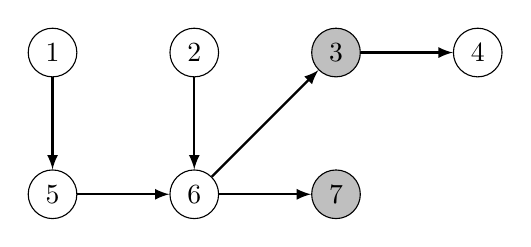
\begin{tikzpicture}[scale=0.9]
\node[draw, circle] (1) at (0,0) {1};
\node[draw, circle] (2) at (2,0) {2};
\node[draw, circle, fill=lightgray] (3) at (4,0) {3};
\node[draw, circle] (4) at (6,0) {4};
\node[draw, circle] (5) at (0,-2) {5};
\node[draw, circle] (6) at (2,-2) {6};
\node[draw, circle, fill=lightgray] (7) at (4,-2) {7};

\path[draw,thick,->,>=latex] (1) -- (5);
\path[draw,thick,->,>=latex] (2) -- (6);
\path[draw,thick,->,>=latex] (3) -- (4);
\path[draw,thick,->,>=latex] (5) -- (6);
\path[draw,thick,->,>=latex] (6) -- (3);
\path[draw,thick,->,>=latex] (6) -- (7);
\end{tikzpicture}
\end{center}

This is a maximum antichain, because it is not possible
to construct any antichain that would contain three nodes.
We have seen before that the size of a minimum
general path cover of this graph consists of two paths.
